\documentclass[a4paper]{ctexart}

\usepackage{tabularx} % extra features for tabular environment
\usepackage{amsmath}  % improve math presentation
\usepackage{graphicx} % takes care of graphic including machinery
\usepackage[margin=1in,letterpaper]{geometry} % decreases margins
\usepackage{cite} % takes care of citations
\usepackage[final]{hyperref} % adds hyper links inside the generated pdf file
\usepackage{ctex}
\usepackage{titlesec}
%\usepackage{CJKutf8, CJK}
\usepackage{makecell}                 % 三线表-竖线
\usepackage{booktabs}                 % 三线表-短细横线
% \usepackage{natbib}
\usepackage{graphicx}				  % 表格单元格逆时针
\usepackage{multirow}				  % 合并单元格
\usepackage{array}
\usepackage{amssymb}				  % 勾
\usepackage{amsmath}
\usepackage{longtable}                % 导入 longtable 宏包,表格自动换行
\usepackage{caption}
\usepackage{subcaption}               % 设置子图
\usepackage{color}					  % 文本颜色包
\usepackage{xcolor}
\usepackage{bbm}					  % 输入指示函数
\usepackage{tablefootnote}			  % 表格注释
\usepackage{pythonhighlight}
%\usepackage{fancyhdr}
\usepackage{lastpage}
\usepackage{tocloft}
\usepackage{authblk}
\usepackage{setspace}

\usepackage[section]{placeins}

% 设置页面边距
\geometry{a4paper, top=1.7cm, bottom=1.6cm, left=1.6cm, right=1.6cm}

%\pagestyle{fancy}
%\fancyhf{}
%\fancyhead{}
%\fancyfoot{}
%\fancyhead[R]{\small Page \thepage\ of \pageref*{LastPage}}
%\fancyhead[L]{\zihao{-5} \songti 开题报告}

\usepackage{listings}                 % 导入代码块
\usepackage{xcolor}
\lstset{
	numbers=left, 
	tabsize=1,
	columns=flexible, 
	numberstyle=  \small, 
	keywordstyle= \color{ blue!70},
	commentstyle= \color{red!50!green!50!blue!50}, 
	frame=shadowbox, % 阴影效果
	rulesepcolor= \color{ red!20!green!20!blue!20} ,
	escapeinside=``, % 英文分号中可写入中文
	xleftmargin=2em,
	xrightmargin=2em, 
	aboveskip=1em,
} 

\hypersetup{
	colorlinks=true,       % false: boxed links; true: colored links
	linkcolor=blue,        % color of internal links
	citecolor=blue,        % color of links to bibliography
	filecolor=magenta,     % color of file links
	urlcolor=blue         
}
%++++++++++++++++++++++++++++++++++++++++
\titleformat{\section}{\Large\bfseries}{\thesection}{1em}{}
\titleformat{\subsection}{\large\bfseries}{\thesubsection}{1em}{}
\titleformat{\subsubsection}{\normalsize\bfseries}{\thesubsubsection}{1em}{}
\titleformat{\paragraph}[runin]{\normalsize\bfseries}{\paragraph}{1em}{}
\titleformat{\subparagraph}[runin]{\normalsize\bfseries}{\subparagraph}{1em}{}

\begin{document}
	
	\title{\songti \zihao{4}一种基于边缘结构指导的弱光图像增强方法}
	\author{\textrm{Ku Jui}}
	\date{\textrm{October 2023}}
	\maketitle
	
	\newpage
	
	% 	\begin{abstract}
		%		In this experiment we studied a very important physical effect by measuring the
		%		dependence of a quantity $V$ of the quantity $X$ for two different sample
		%		temperatures.  Our experimental measurements confirmed the quadratic dependence
		%		$V = kX^2$ predicted by Someone's first law. The value of the mystery parameter
		%		$k = 15.4\pm 0.5$~s was extracted from the fit. This value is
		%		not consistent with the theoretically predicted $k_{theory}=17.34$~s. We attribute %this
		%		discrepancy to low efficiency of our $V$-detector.
		%	\end{abstract}
	\renewcommand{\contentsname}{目录}
	\renewcommand{\cfttoctitlefont}{\hfill\Large\bfseries}
	\renewcommand{\cftaftertoctitle}{\hfill}
	\renewcommand{\tablename}{表}
	\renewcommand{\figurename}{图}
	
	\numberwithin{equation}{section}
	
	\tableofcontents  % 自动生成目录
	
	\newpage
	
	\section{立题依据}
	
	\subsection{课题的研究意义}
	
	弱光图像增强(Low-light image enhancement, LLIE)是图像处理中的一个重要任务,其目标是提升在低光环境下拍摄的图像的感知质量。这个领域的近期进展主要由深度学习方法主导,包括不同的学习策略、网络架构、损失函数和训练数据。
	
	低光图像增强在不同领域享有广泛的应用,包括视觉监控、自动驾驶和计算摄影。特别是,智能手机摄影已经变得无处不在和突出。受限于相机光圈的大小、实时处理的要求以及存储器的约束,在昏暗环境中用智能手机的相机拍摄照片尤其具有挑战性。
	
	用于低光增强的传统方法包括基于直方图均衡的方法和基于 Retinex 模型的方法。然而,这些方法存在一些局限性,例如在 Retinex 模型中通常忽略噪声\cite{liu2021retinex, xu2020learning},因此在增强结果中保留或放大噪声;找到有效的先验或正则化是具有挑战性的,不准确的先验或正则化可能导致增强结果中的伪像和颜色偏差;由于其复杂的优化过程,运行时间相对较长。
	
	近年来基于深度学习的 LLIE 取得了引人注目的成功。基于深度学习的解决方案比传统方法具有更好的准确性、鲁棒性和速度,因此越来越受到关注。然而,现有的低光照图像增强技术聚焦于构建数据驱动的深度网络,通常其网络模型复杂,导致计算效率低、推理速度慢,并且由于对于训练数据分布的依赖性导致其在未知场景下的性能缺乏保障。
	
	为了解决这些问题并推动该领域的发展,研究者们提出了一些新颖的方法和工具。例如,他们提出了一个大尺度低光图像与视频数据集,并开发了一个包含多种主流 LLIE 方法的在线平台。这些工具可以帮助研究者和开发者更好地理解和改进现有技术,并为未来研究提供宝贵资源。
	
	\subsection{国内外研究现状分析}
	
	\subsubsection{传统弱光图像增强方法}
	基于传统方法的弱光图像增强算法通常利用单张图像自身的性质进行图像增强。主要包括灰度变换(GT)\textcolor{blue}{\cite{ueng1995gamma}}、直方图均衡化(HE)\textcolor{blue}{\cite{stark2000adaptive}}、Retinex模型\textcolor{blue}{\cite{land1971lightness}}、频域处理\textcolor{blue}{\cite{liu2021benchmarking}}、图像融合模型\textcolor{blue}{\cite{dai2019fractional}}、去雾模型\textcolor{blue}{\cite{ma2019improved}}等。
	
	基于 Retinex 理论的方法在弱光图像增强领域非常受欢迎。传统Retinex算法改善图像质量,但存在颜色失真和光晕问题。针对这些缺陷,文献\cite{cooper2004analysis}提出的算法能提高对比度和亮度,但在天空部分可能产生不自然的颜色和伪影。直方图均衡化\cite{stark2000adaptive}通过重新调整图像的直方图分布来增加全局对比度,但可能导致背景噪声和降低有用图像内容的对比度。此外,直方图均衡化无法适用于复杂低光照场景。基于图像反相的方法\cite{dong2010fast}利用低光照图像的反相与有雾图像的相似性,但容易导致增强结构出现黑边。
	
	\subsubsection{基于深度学习的弱光图像增强方法}
	
	自2017年LLNet\cite{lore2017llnet}的出现以来,基于深度学习的弱光图像增强方法备受关注。到2023年,已经涌现出上百种方法,显示出深度学习在准确性、鲁棒性和速度方面的优势。这些方法可分为有监督学习、无监督学习、半监督学习、零采样学习。
	
	有监督学习依赖标记的数据集,分为端到端和Retinex理论方法。LLNet和MBLLEN\cite{lv2018mbllen}是早期方法,而GLADNet\cite{wang2018gladnet}、TBEFN\cite{lu2020tbefn}、PRIEN\cite{li2021low}和C-LIENet\cite{ravirathinam2021c}采用了不同的策略。与传统端到端方法相比,融合深度学习与Retinex理论的方法在某些情况下表现更优越。RetinexNet\cite{wei2018deep}和MSR-net\cite{shen2017msr}结合了数据驱动和Retinex理论,取得了良好效果。EnlightenGAN\cite{jiang2021enlightengan}是首个成功应用非配对训练的例子,采用全局-局部判别器结构和自特征保留损失。LE-GAN\cite{fu2022gan}使用不变身份损失和注意力模块,构建了一个较大的非配对弱光图像数据集PNLI。HEP\cite{zhang2021unsupervised}采用直方图均衡化的无监督增强方法,通过噪声分离模块提高图像纹理信息和亮度细节。半监督学习结合了监督学习和非监督学习的优点。DRBN\cite{qiao2021deep}采用深度递归频带网络,优化频带表示以去除噪声。HybridNet\cite{robert2018hybridnet}分为有监督和无监督分支,有效地训练分类器。零采样学习无需预先训练的数据集,Zhu\cite{zhu2020zero}的RRDNet通过三分支全卷积神经网络处理低光照图像,成功去除噪声。ExCNet\cite{zhang2019zero}通过估计最适合当前背光图像的参数曲线,在复杂拍摄环境中进行实时图像增强。
	
	此外,以 Vision Transformer(ViT)\cite{dosovitskiy2020image}为核心的监督学习任务受到广泛关注。在这一领域中,Cui等人\cite{cui2022illumination}开发了一种名为照明自适应变压器 (Illumination-Adaptive Transformer, \textbf{IAT}) 的网络。这个网络是全监督训练模式下的超轻量级架构。它借鉴了目标检测网络 \textbf{DETR} (Detection Transformer)的设计理念\cite{carion2020end},实现了一个端到端的变压器结构,有效地解决了弱光环境下的视觉效果问题。IAT网络的主要优点在于其出色的性能和快速的处理速度。另一方面,Wang等人\cite{wang2023ultra}提出了一种新型的弱光变压器网络,名为\textbf{LLFormer}。LLFormer的关键特性是其基于轴的多头自注意力和跨层注意力融合块,这大大减少了计算的复杂度。此外,Wang等人还创建了一个4K和8K超高清图像(UHD-LOL)的基准数据集,用以评估LLFormer的性能。这代表了首次尝试解决超高清弱光图像增强(UHD-LLIE)的任务。
	
	\subsection{主要的参考文献}
	
	\renewcommand{\refname}{}
	
	\vspace{-1cm}
	
	\bibliographystyle{unsrt}
	\bibliography{reference}
	
	\section{研究方案}
	
	\subsection{研究目标}
	
	现有的方法仍有很大的改进空间,例如如何在提高亮度的同时消除产生的噪声,如何避免颜色失真现象等。一些现有的方法可以有效地解决一个问题,但往往会忽略了其他问题。不同的方法在不同的数据集上往往具有不同的优势,即在不同的评估标准下有不同的优势,如图\ref{fig: VE-LOL-L Visual}展示了不同算法在VE-LOL-L数据集\cite{liu2021benchmarking}下的可视化结果。
	
	\begin{figure}[htbp]
		\centering
		\begin{subfigure}{0.17\columnwidth}
			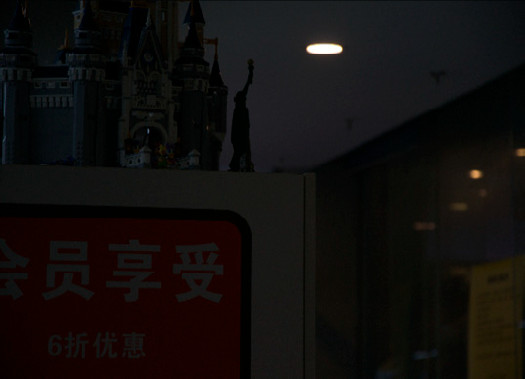
\includegraphics[width=\linewidth]{picture/LLIE/VE-LOL-L/input}
			\captionsetup{font=scriptsize}
			\caption*{input \\ \quad }
			\label{fig: input}
		\end{subfigure}
		\begin{subfigure}{0.17\columnwidth}
			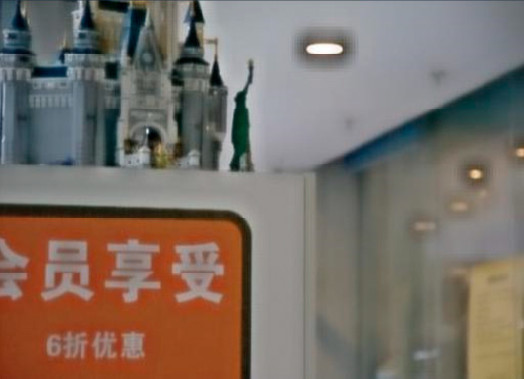
\includegraphics[width=\linewidth]{picture/LLIE/VE-LOL-L/LLNet}
			\captionsetup{font=scriptsize}
			\caption*{LLNet \\ (2017)}
			\label{fig: LLNet_VE_LOL}	
		\end{subfigure}
		\begin{subfigure}{0.17\columnwidth}
			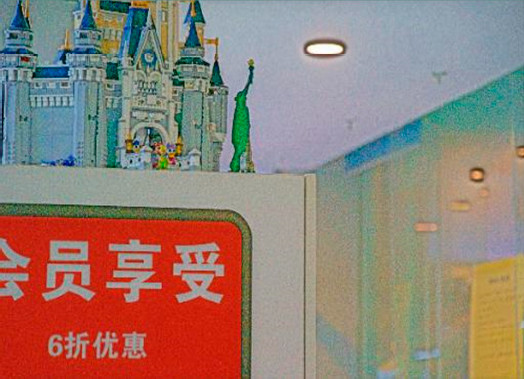
\includegraphics[width=\linewidth]{picture/LLIE/VE-LOL-L/RetinexNet}
			\captionsetup{font=scriptsize}
			\caption*{RetinexNet \\ (2018)}
			\label{fig: RetinexNet_VE_LOL}	
		\end{subfigure}
		\begin{subfigure}{0.17\columnwidth}
			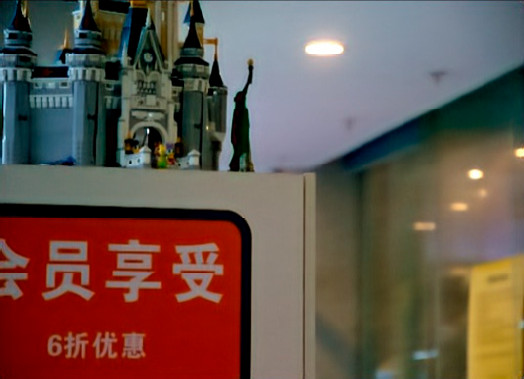
\includegraphics[width=\linewidth]{picture/LLIE/VE-LOL-L/MBLLEN}
			\captionsetup{font=scriptsize}
			\caption*{MBLLEN \\ (2018)}
			\label{fig: MBLLEN_LOL}	
		\end{subfigure}
		\begin{subfigure}{0.17\columnwidth}
			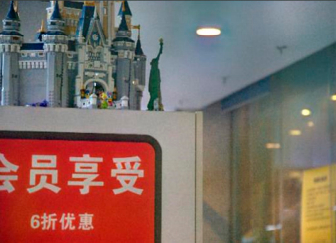
\includegraphics[width=\linewidth]{picture/LLIE/VE-LOL-L/EnlightenGAN}
			\captionsetup{font=scriptsize}
			\caption*{EnlightenGAN \\ (2019)}
			\label{fig: EnlightenGAN_VE_LOL}	
		\end{subfigure}
		\begin{subfigure}{0.17\columnwidth}
			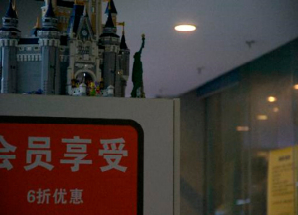
\includegraphics[width=\linewidth]{picture/LLIE/VE-LOL-L/RRDNet}
			\captionsetup{font=scriptsize}
			\caption*{RRDNet \\ (2020)}
			\label{fig: RRDNet_VE_LOL}	
		\end{subfigure}
		\begin{subfigure}{0.17\columnwidth}
			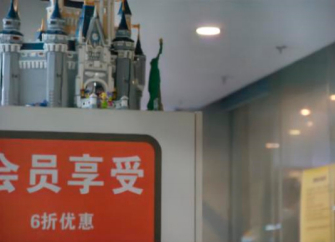
\includegraphics[width=\linewidth]{picture/LLIE/VE-LOL-L/DRBN}
			\captionsetup{font=scriptsize}
			\caption*{DRBN \\ (2020)}
			\label{fig: DRBN_VE_LOL}	
		\end{subfigure}
		\begin{subfigure}{0.17\columnwidth}
			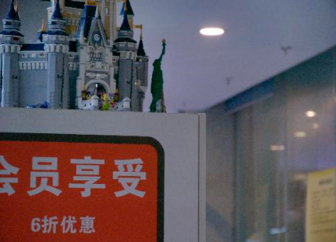
\includegraphics[width=\linewidth]{picture/LLIE/VE-LOL-L/Zero-DCE++}
			\captionsetup{font=scriptsize}
			\caption*{Zero-DCE++ \\ (2021)}
			\label{fig: Zero-DCE++}	
		\end{subfigure}
		\begin{subfigure}{0.17\columnwidth}
			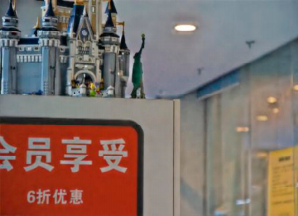
\includegraphics[width=\linewidth]{picture/LLIE/VE-LOL-L/KinD++}
			\captionsetup{font=scriptsize}
			\caption*{KinD++ \\ (2021)}
			\label{fig: KinD++}	
		\end{subfigure}
		\begin{subfigure}{0.17\columnwidth}
			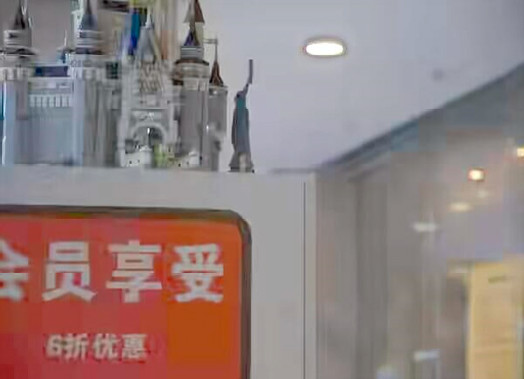
\includegraphics[width=\linewidth]{picture/LLIE/VE-LOL-L/URetinexNet}
			\captionsetup{font=scriptsize}
			\caption*{URetinexNet \\ (2022)}
			\label{fig: URetinexNet}	
		\end{subfigure}
		\caption{
			\label{fig: VE-LOL-L Visual} 
			不同算法对从 VE-LOL-L 数据集采样的弱光图像的可视化结果。 
		}
	\end{figure}
	
	近年来,基于深度学习的低光图像增强(LLIE)技术取得了显著成就,它使用神经网络来学习从弱光图像到自然光图像的映射。与传统方法相比,基于深度学习的解决方案在准确性、鲁棒性和处理速度方面表现更优,因此受到了广泛关注。特别是卷积神经网络(CNN)在多个计算机视觉任务中展现出卓越的性能。CNN通过利用注意力机制和\cite{yang2021locally, zhang2020attention}上下文信息,能够从原始图像中有效提取多尺度特征\cite{li2018multi, zamir2020learning}。在这些成果的推动下,基于CNN的低光图像增强方法得到了持续发展。例如,一种基于CNN的自适应低光图像增强框架\cite{li2020visual}显著提升了图像的对比度、颜色和细节信息。然而,现有的基于CNN的方法大多集中于图像亮度、纹理和颜色的恢复,对于局部光照不均匀、颜色信息和细节信息的丢失问题,仍存在过增强或增强不足的挑战。
	
	现有的方法可能无法在极暗或极亮的区域恢复图像边缘细节\cite{xu2023low},如图\ref{fig: SNR (CVPR 2022)}和图\ref{fig: SMG-LLIE}所示,暗区结构细节模糊。同时,当物体边缘不清晰时,像素级损失往往会模糊边缘,破坏图像细节。而加入边缘先验可以降低优化外观重构时的不适定程度。人类视觉系统对边缘高度敏感,保留结构信息对图像重建任务的性能至关重要。定义边缘可以通过学习区分黑暗区域的不同物体来指导增强过程,而不仅仅是识别低光区域。通过保留图像中的结构属性,这使得物体之间的可见性更好。
	
	\begin{figure}[htb]
		\centering
		\begin{subfigure}{0.45\columnwidth}
			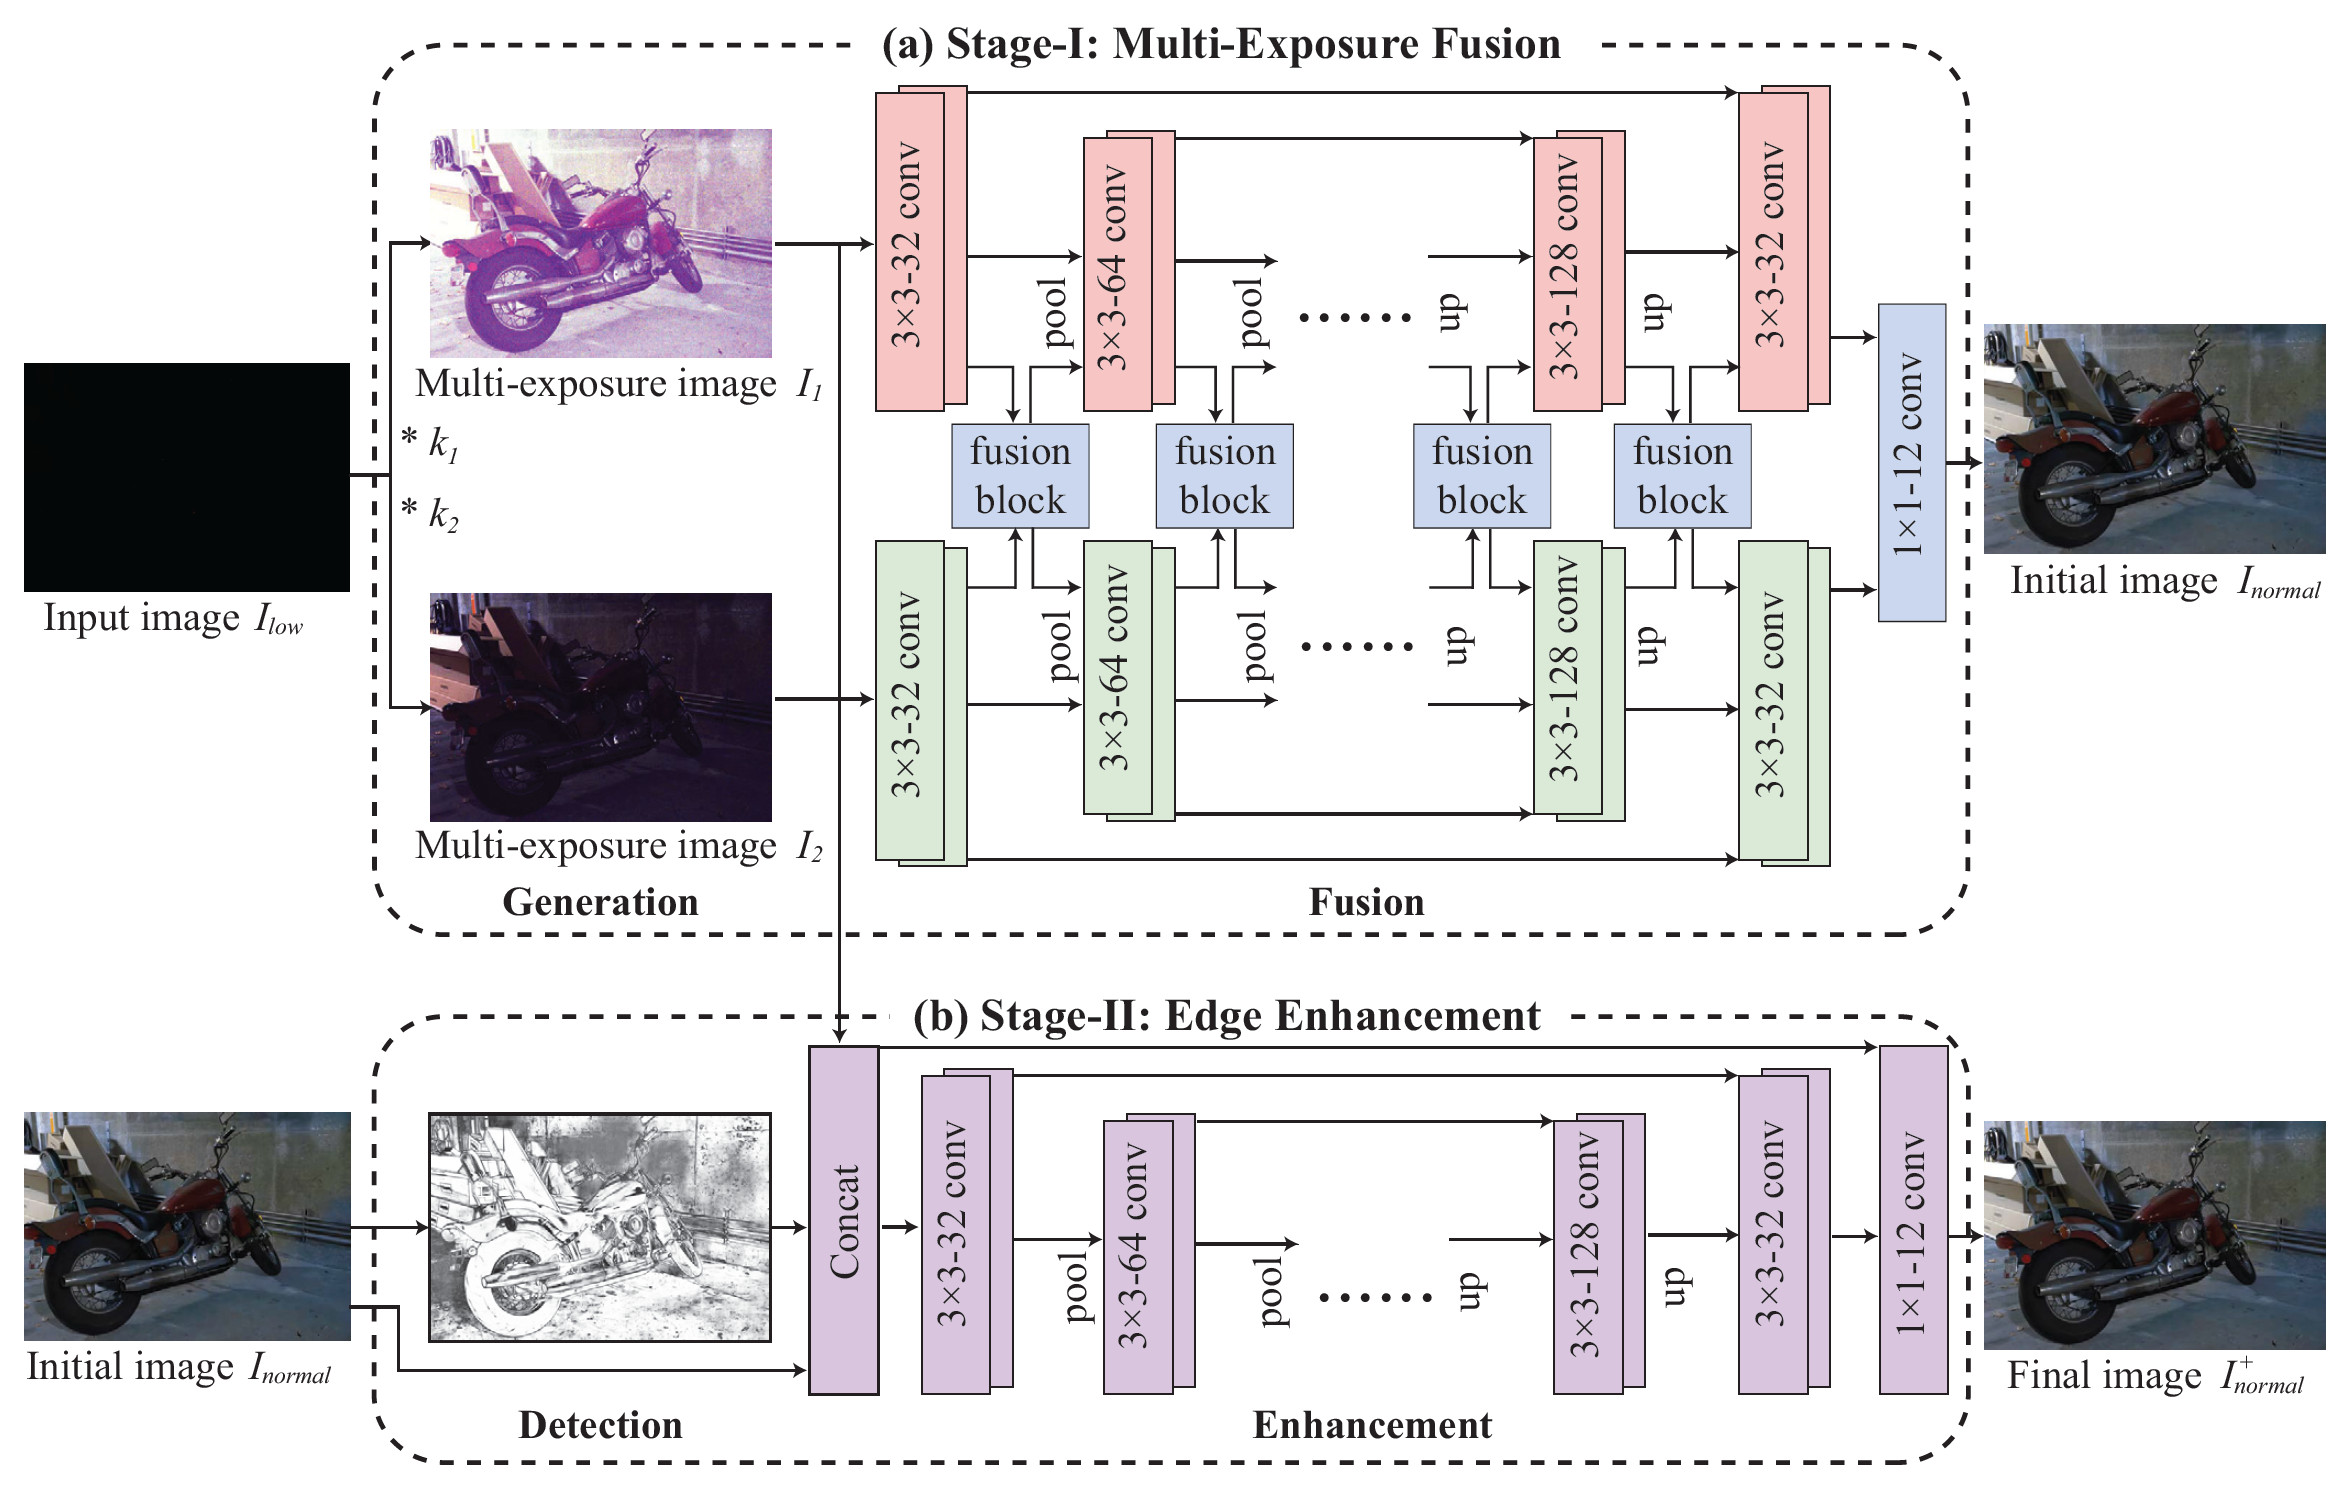
\includegraphics[width=\linewidth]{picture/LLIE/EEMEFN/EEMEFN framework}
			\captionsetup{font=scriptsize}
			\caption{\label{fig: EEMEFN}
				该 LLIE 结构源自\cite{zhu2020eemefn},如其 Multi-Exposure Fusion 部分采用多曝光融合结构,与由 Initial image 生成的边缘图进行 Concat, 后续通过一个 U-Net 网络进一步恢复图像。}
		\end{subfigure}
		\begin{subfigure}{0.45\columnwidth}
			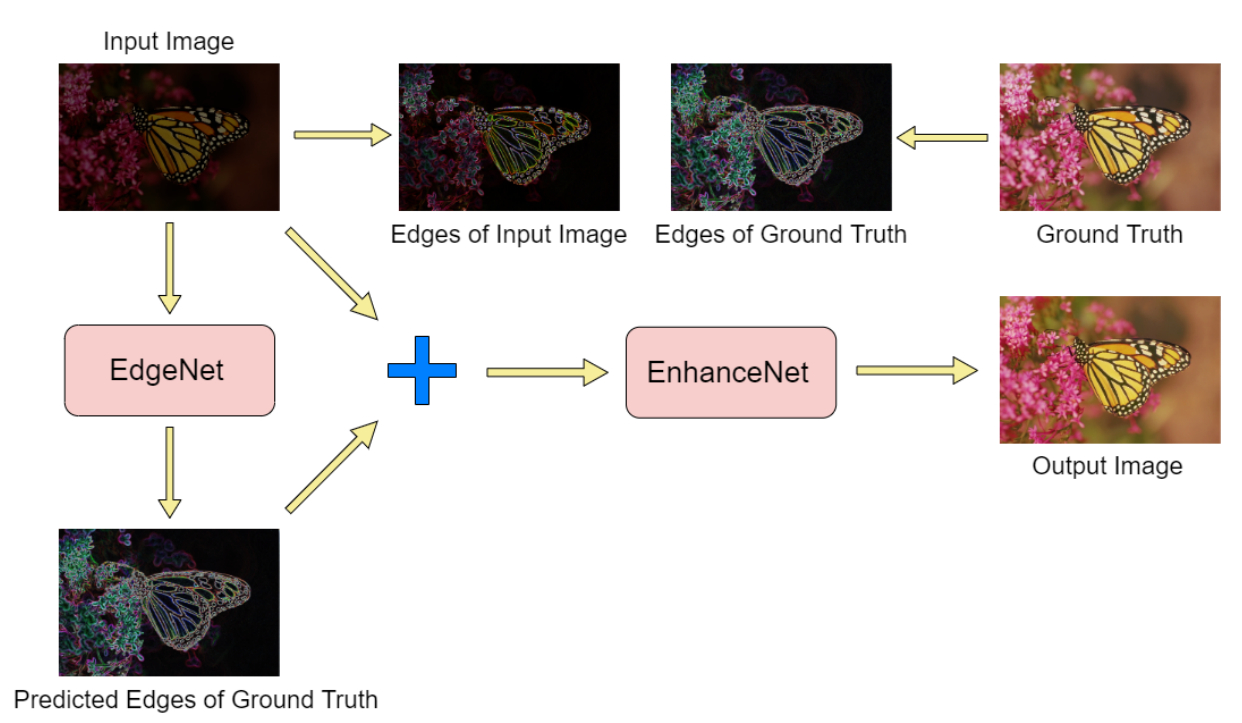
\includegraphics[width=\linewidth]{picture/LLIE/EdgeNet/Archtecture workflow}
			\captionsetup{font=scriptsize}
			\caption{\label{fig: EdgeNet} 
				该 LLIE 结构源自\cite{rana2021edge}使用 EdgeNet 首先从低光图像中过滤边缘,EnhanceNet 反复使用上采样和下采样块的组合,从局部到全局逐渐提取特征,并消除伪影和噪声。}
		\end{subfigure}
		\caption{
			\label{fig: Traditional Architecture}
			边缘图像指导弱光图像增强的传统架构。
		}
	\end{figure}
	\FloatBarrier

	\begin{figure}[htb]
		\centering
		\begin{subfigure}{0.25\columnwidth}
			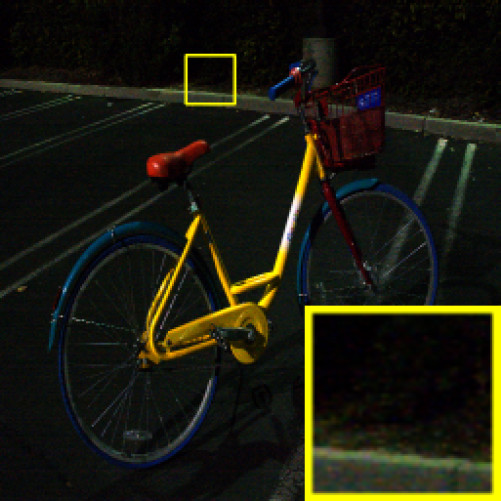
\includegraphics[width=\linewidth]{picture/LLIE/Structure Modeling and Guidance/Input}
			\captionsetup{font=scriptsize}
			\caption{Input}
			\label{fig: Input}
		\end{subfigure}
		\begin{subfigure}{0.25\columnwidth}
			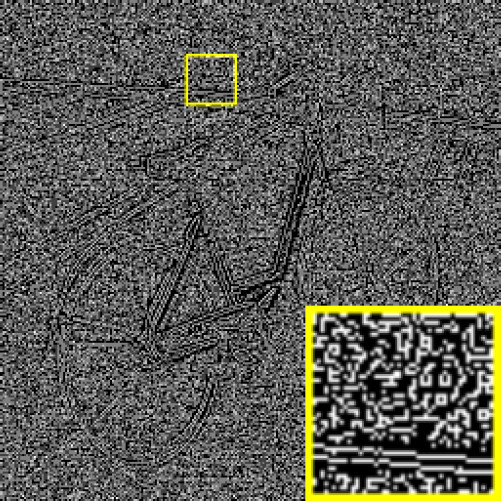
\includegraphics[width=\linewidth]{picture/LLIE/Structure Modeling and Guidance/Structure of (a)}
			\captionsetup{font=scriptsize}
			\caption{Structure of (a)}
			\label{fig: Structure of (a)}	
		\end{subfigure}
		\begin{subfigure}{0.25\columnwidth}
			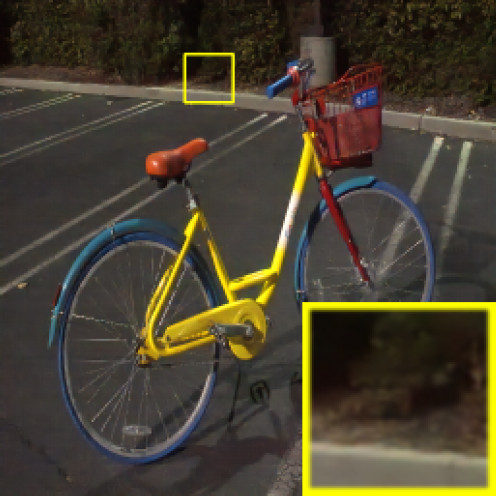
\includegraphics[width=\linewidth]{picture/LLIE/Structure Modeling and Guidance/SNR (CVPR 2022)}
			\captionsetup{font=scriptsize}
			\caption{SNR (CVPR 2022)}
			\label{fig: SNR (CVPR 2022)}	
		\end{subfigure}
		\begin{subfigure}{0.25\columnwidth}
			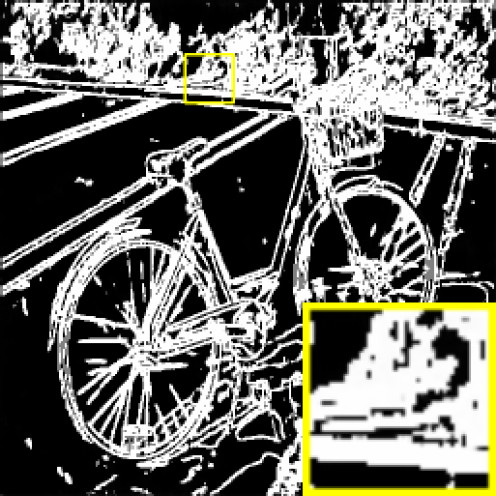
\includegraphics[width=\linewidth]{picture/LLIE/Structure Modeling and Guidance/Structure Modeling}
			\captionsetup{font=scriptsize}
			\caption{Structure Modeling}
			\label{fig: Structure Modeling}
		\end{subfigure}
		\begin{subfigure}{0.25\columnwidth}
			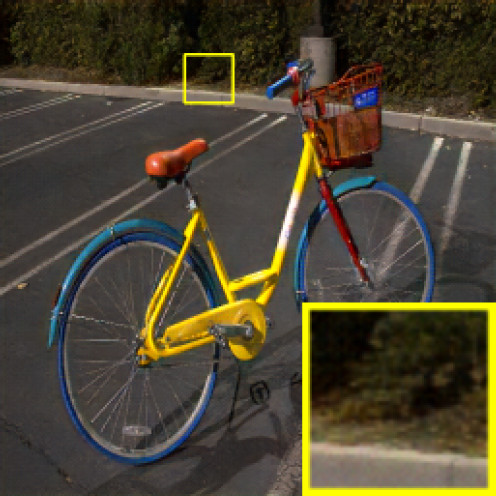
\includegraphics[width=\linewidth]{picture/LLIE/Structure Modeling and Guidance/Ours}
			\captionsetup{font=scriptsize}
			\caption{SMG-LLIE}
			\label{fig: SMG-LLIE}
		\end{subfigure}
		\begin{subfigure}{0.25\columnwidth}
			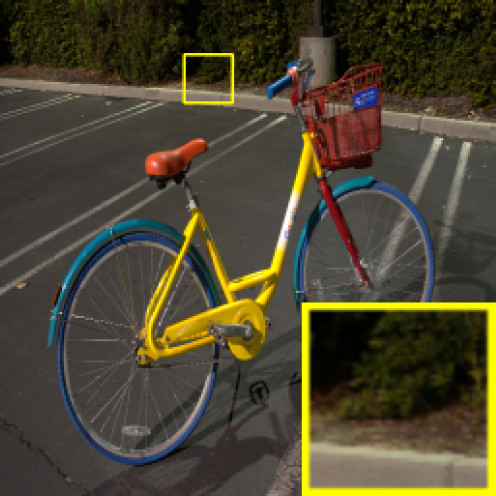
\includegraphics[width=\linewidth]{picture/LLIE/Structure Modeling and Guidance/Ground Truth}
			\captionsetup{font=scriptsize}
			\caption{Ground Truth}
			\label{fig: Ground Truth}
		\end{subfigure}
		\caption{
			\label{fig: Structural Information}
			SID-sRGB\cite{chen2018learning}中一张弱光图片, 通过SOTA方法 (c) 和\cite{xu2023low}提出的方法 (e)增强。作者的方法可以从输入的图像中合成结构图(d),使细节更清晰,对比度更清晰,颜色更鲜艳。虽然(c)的 PSNR 为 28.17,但其 SSIM 低为 0.75。作者的方法在dB和SSIM\cite{wang2004image}的得分都很高,分别为28.60 dB 和 0.80。
		}
	\end{figure}
	\FloatBarrier
	
	基于这个问题,即\textbf{如何更好的使用边缘图来“指导”弱光图像的恢复?}我们对此进行了相关文献调研。其中,一类方法(如图\ref{fig: Traditional Architecture}所示,我们称之为传统架构)是采用边缘检测思想来引导弱光图像增强,其策略是将边缘图与\textbf{一张从弱光中初步恢复的图像}(后面统一称作初步恢复图像)进行串联,然后通过一个增强网络来实现最终的图像增强\cite{zhu2020eemefn, rana2021edge}。但是我们通过观察这类模型的架构发现其具有以下三个特点:

	\begin{itemize}
		\item [(1)] 其恢复结果的质量往往会受到最后的增强网络设计和初步恢复图像所包含特征与真实图像特征之间的相似度的影响。
		
		\item [(2)] 边缘图的准确性会极大影响最终的恢复结果,直接从弱光图像中获取边缘图具有一定的挑战性。
		
		\item [(3)] 边缘图与初步恢复图像之间多采用串联方式输入卷积以获得最终增强结果。
	\end{itemize}
	
	传统架构存在一定的局限性,虽然采用了边缘结构信息增强弱光图像,但是无法很好的利用边缘信息语义指导恢复弱光图像,需要在现有的直接串联方法的基础上进行改进。此外,从低光照中的图片很难提取到好的结构信息,如何设计更好的边缘网络从弱光图像中提取出接近 GT 边缘图的结果是我们需要考虑的问题。
	
	作者\cite{xu2023low}提出了一种基于结构先验的图像增强方式,以更好的从弱光图像中提取到更有效的边缘信息并用于指导图像增强。从图\ref{fig: Structural Information}和\ref{fig: LLI Structure Information}中可以看到边缘图和LBP图\cite{pietikainen2010local}所反映结构信息具有明显的区别,边缘信息能反映更多的细节信息。我们不难发现,相较于LBP,图像边缘图仅保留了很少的数据量,其剔除了不相关的信息,保留了图像重要的结构属性。人类视觉系统对边缘高度敏感,保留结构信息对图像重建任务的性能至关重要。定义边缘可以通过学习区分黑暗区域的不同物体来指导增强过程,而不仅仅是识别低光区域。通过保留图像中的结构属性,这使得物体之间的可见性更好。
	
	\subsection{研究内容}
	
	综上所述,本研究旨在实现以下明确的研究目标:
	
	\begin{itemize}
		\item [(1)] \textbf{边缘网络的开发:} 设计并构建一个创新的边缘网络,其核心功能是从低光照图像中直接提取边缘结构图。该网络生成的结构图应与 GT 生成的边缘结构图具有高度的相似性,从而确保准确性和可靠性。
		
		\item [(2)] \textbf{初步恢复图像的生成模型:} 开发一个用于生成初步恢复图像的低光照图像增强模型。该模型应专注于从弱光条件下的图像中恢复清晰度和细节,以提高整体图像质量。
		
		\item [(2)] \textbf{边缘语义信息引导的增强模型:} 在现有的直接串联方法基础上,进行创新性改进,构建一种更有效利用边缘语义信息的增强网络模型。目的在于通过这种改进,进一步提升图像增强过程中边缘结构的利用效率和效果。
	\end{itemize}
	
	通过实现这些目标,本研究期望对弱光图像处理领域的理论与实践作出贡献,特别是在图像边缘结构的提取和利用方面。
	
	\subsection{拟解决的关键问题}
	
	在弱光图像增强(Low-Light Image Enhancement, LLIE)领域的研究中,目前存在几个主要的技术挑战,它们分别涉及噪声和伪影抑制、颜色保真度和边缘细节恢复。这些挑战如下所述:
	
	\begin{itemize}
		\item [(1)]
		\textbf{噪声放大问题:}在提升图像亮度的过程中,现有的增强方法常常导致噪声的显著放大,而这些方法在有效抑制放大噪声方面表现不佳。这一问题尤其在高ISO值或低光照条件下拍摄的图像中更为明显。
		\item [(2)]
		\textbf{颜色失真:}多数现有方法在增强过程中难以保持原始颜色的真实性,导致颜色失真。这种失真可能表现为色彩偏移或不自然的色彩饱和度,从而降低了图像的视觉质量。
		
		\item [(3)]
		\textbf{边缘细节恢复不足:}在极暗或极亮区域,当前的LLIE方法往往无法有效恢复图像边缘细节。这限制了图像在细节丰富度和空间分辨率方面的表现,尤其是在需要精细纹理和清晰边界的应用场景中。
		
	\end{itemize}

	\subsection{拟采取的研究方法}
	
	在探索弱光图像增强的研究方法时,我们综合考虑了不同的深度学习网络结构,以提高模型对低光条件下图像的表现。以下是我们采取的主要研究方法。
	
	在计算机视觉中,注意力机制是常用的方法,用于使模型集中于图像关键部分。通常分为基于通道的注意力机制(如Squeeze-and-Excite)和基于空间的注意力机制\cite{woo2018cbam}。然而,这些方法存在卷积远距离特征较差、计算成本高、信息浪费和注意力减弱等限制。针对这些问题,一些研究采用纯注意模型\cite{ramachandran2019stand}和轻量级的通用注意模型CBAM\cite{woo2018cbam}来增强网络表达能力。
	
	U-Net网络在图像语义分割领域取得成功,特别在弱光图像增强方面\cite{chen2018learning}。改进的U-Net++\cite{zhou2018unet++,zhou2019unet++}通过嵌套的密集跳跃连接加强了特征信息融合。尽管基于U-Net的方法在弱光图像增强中取得良好效果,但存在跳过连接仅融合相同尺度特征和全局上下文信息相对稀缺的问题。近期研究尝试通过增加全局信息感知模块(GIA)来改善这些问题\cite{meng2020gia}。
	
	CNN在计算机视觉任务中取得显著结果,尤其在图像亮度、纹理和颜色恢复方面\cite{xu2020learning}。然而,现有CNN方法更注重局部信息,容易在弱光照条件下导致颜色和细节信息损失。
	
	Transformer架构\cite{vaswani2017attention}在图像处理中表现出色,但计算复杂度较高\cite{dosovitskiy2020image}。一些研究通过引入局部窗口策略和与CNN模块的耦合来缓解计算负担\cite{chen2023cross}。这种串联策略旨在充分发挥CNN的平移不变性和局部性,使其与Transformer优势互补。
	
	\subsection{技术路线}

	根据当前文献研究,在低光照图像增强(LLIE)任务中,一种常见方法是采用边缘检测思想来引导弱光图像增强。该策略涉及将边缘图与初步恢复的图像进行串联,随后通过单一的增强网络来实现最终的图像恢复。然而,恢复结果的质量常受最后的增强网络设计以及初步恢复图像所包含特征与真实图像特征相似度的影响。综合目前文献调研发现,目前这类方法生成的图像仍然存在明显噪点。
	
	本研究基于上述的策略,基于边缘结构图来引导弱光图像恢复。通过利用边缘结构图引导图像恢复过程,旨在改善低光照条件下的图像质量,特别是在边缘细节方面。该策略基于深度学习技术和图像处理理论,尤其是边缘检测和图像增强技术。通过这一新方法,我们期望能够克服当前方法中存在的图像噪点问题,提升弱光图像增强的效果。
	
	\begin{figure}[htb]
		\centering 
		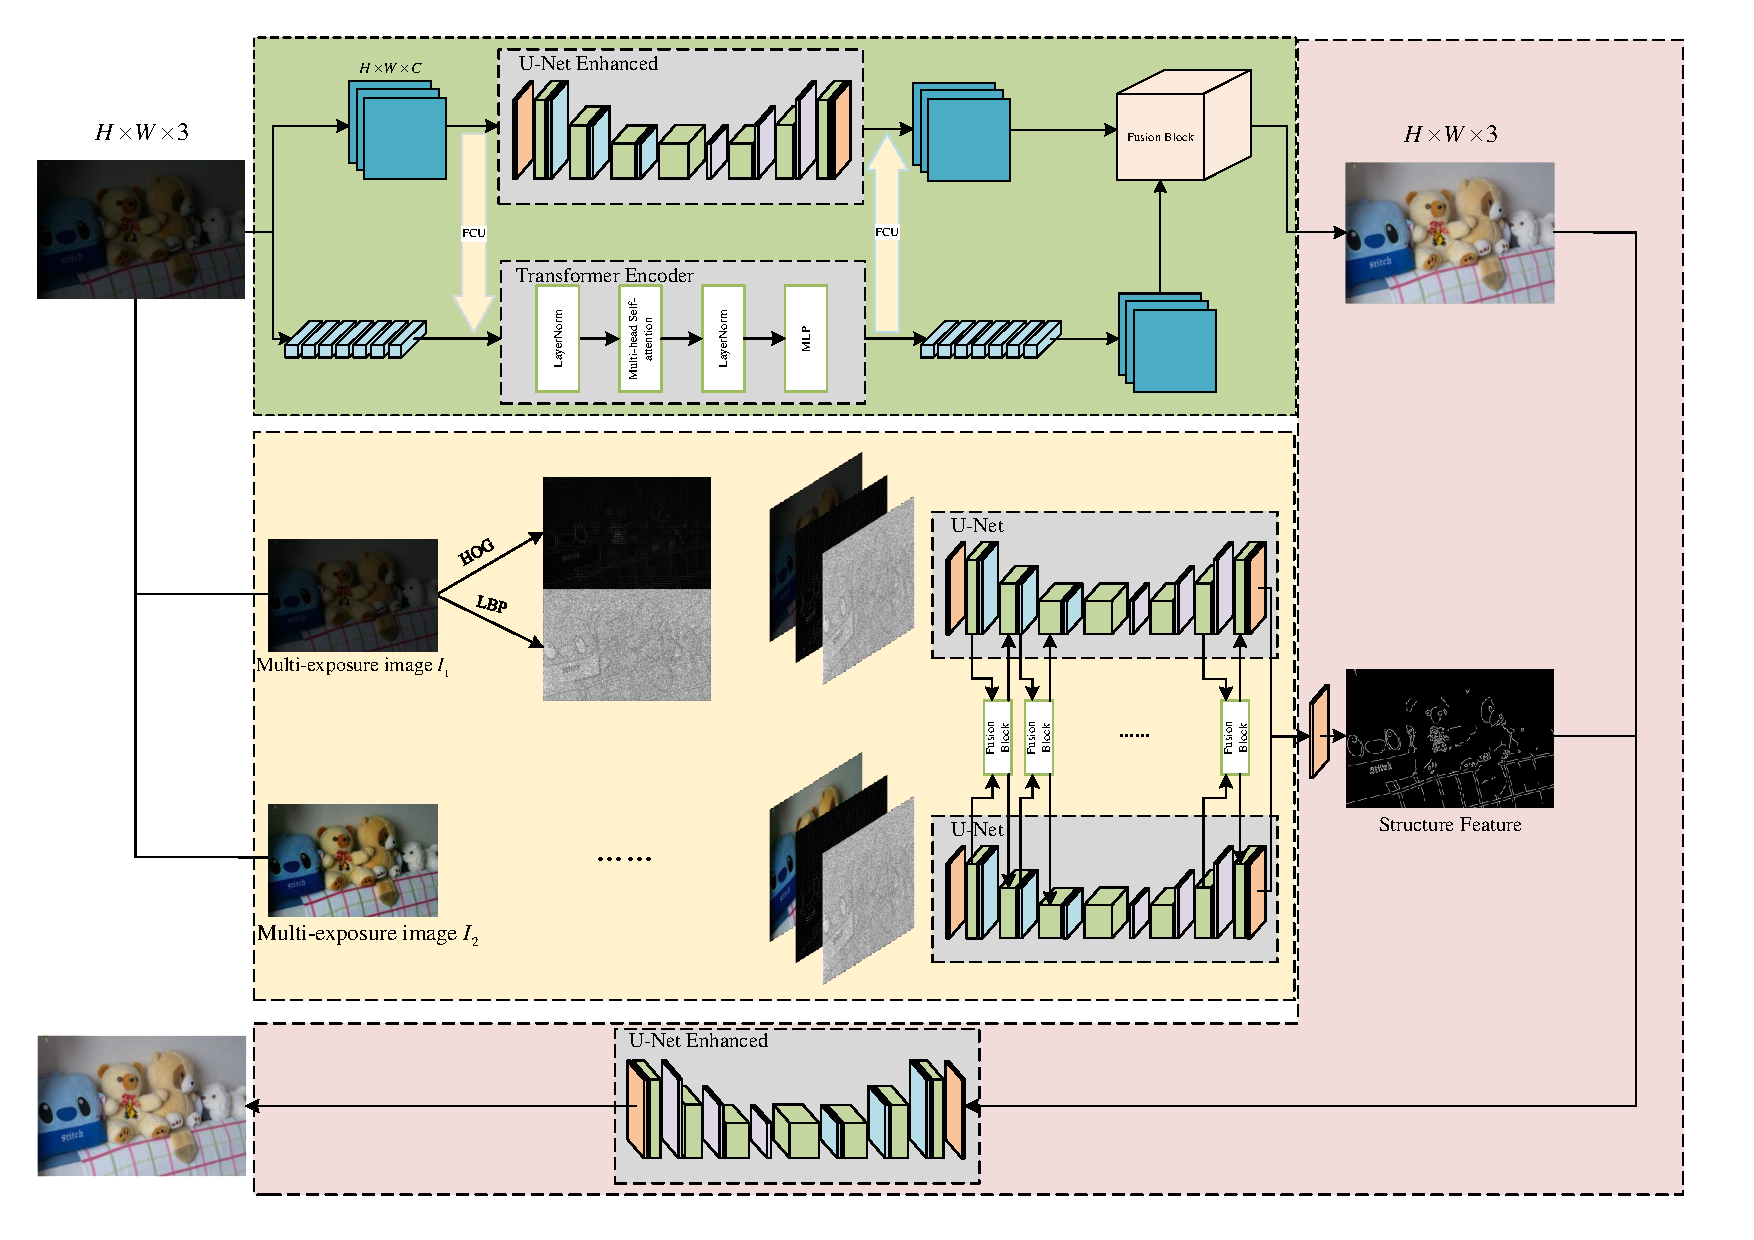
\includegraphics[width=\columnwidth]{picture/LLIE/My Architecture/Total architecture}
		\caption{
			\label{fig: Total Architecture} 
			我们提出的技术框架。
		}
	\end{figure}
	\FloatBarrier
	
	\subsection{方案及可行性研究}
	
	\subsubsection{初步恢复图像的生成模型}
	
	\textbf{初步恢复图像的生成模型}目前主要包括以下几种:
	
	\begin{itemize}
		\item[(1)] 
		多曝光图像融合技术(Multi-exposure Image Fusion, MEF):这种技术涉及获取一系列具有不同曝光度的图像,随后利用图像融合技术以及恢复网络来实现图像的初步恢复。这种方法的优势在于能够从多个曝光级别中综合信息,从而增强图像的细节和动态范围\cite{burt1984pyramid}。
		
		\item[(2)]
		结合卷积神经网络(CNN)与Transformer架构:此方法包括类似于Uformer\cite{wang2022uformer}的串行架构,以及类似于Conformer的并行架构。在我们提出的CNN和Transformer并行架构中(如图\ref{fig: First Architecture}所示),两种架构共同工作以优化图像恢复过程,利用CNN的空间特征提取能力和Transformer的全局信息处理能力。
		
		\item[(3)]
		通过U-Net架构进行弱恢复:使用U-Net架构进行弱光图像的初步恢复,这是一种基于深度学习的方法。U-Net架构因其有效的特征提取和上下文信息融合能力而广泛用于图像处理任务,尤其是在图像分割和恢复领域表现出色。
	\end{itemize}	
	
	\begin{figure}[htb] 
		\centering 		
		\begin{subfigure}{\textwidth}
			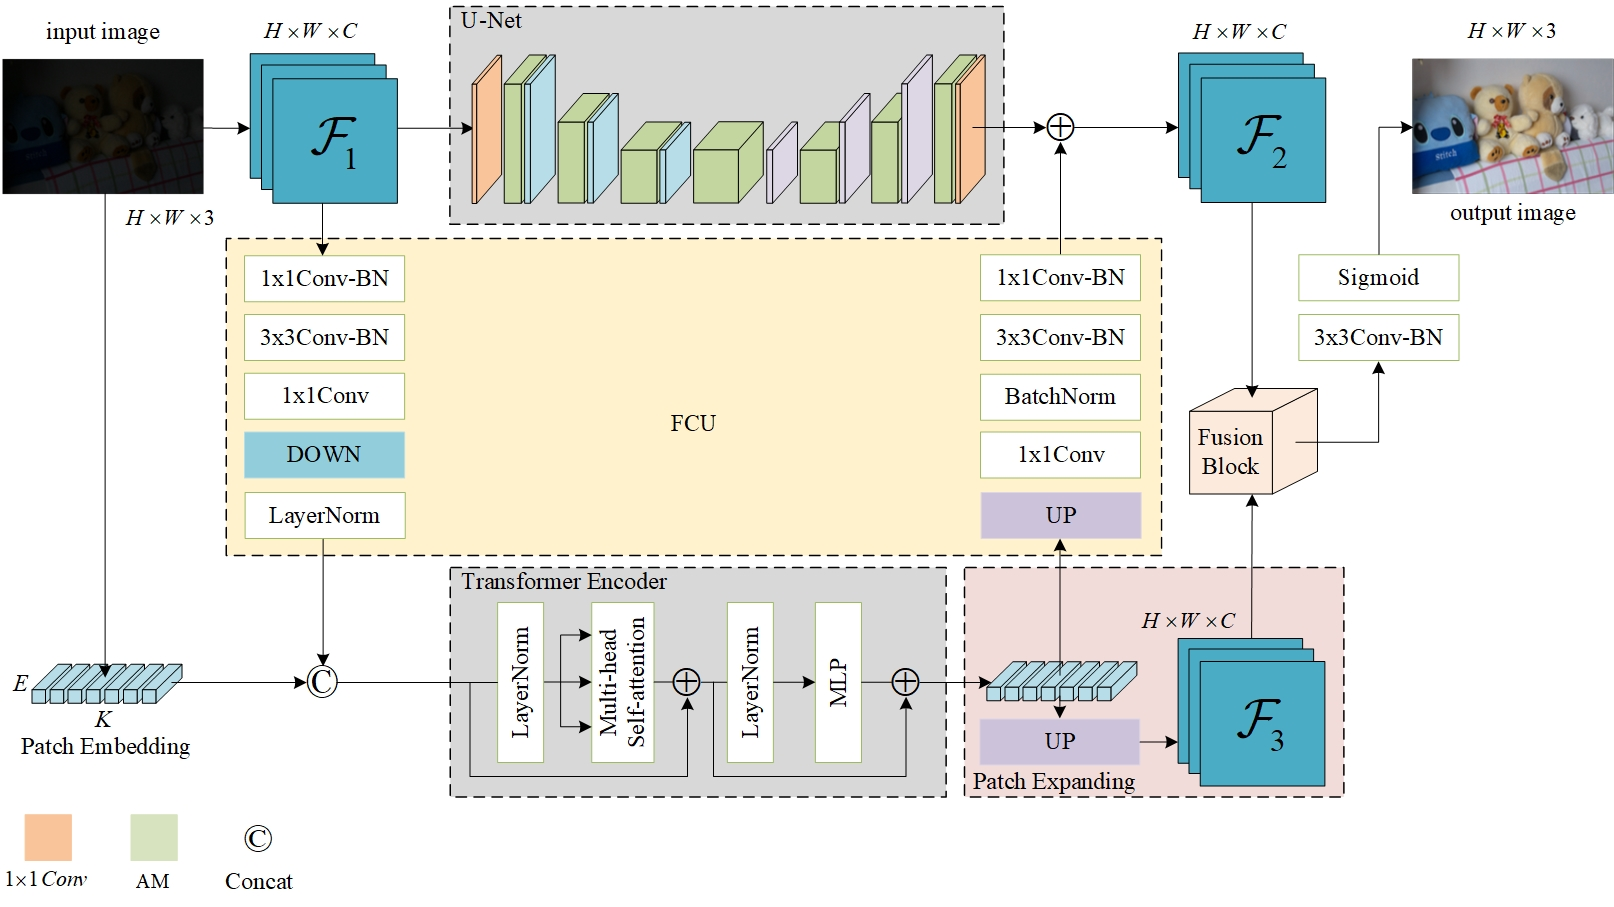
\includegraphics[width=\linewidth]{picture/LLIE/My Architecture/The proposed initial architecture.jpg}
			\captionsetup{font=scriptsize}
			\caption{Parallel Architecture}
			\label{fig: First Architecture}
		\end{subfigure}\\
		\begin{subfigure}{0.4\textwidth}
			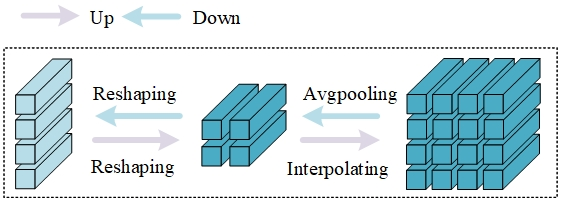
\includegraphics[width=\linewidth]{picture/LLIE/My Architecture/Up-sampling and down-sampling}
			\captionsetup{font=scriptsize}
			\caption{Up-sampling and Down-sampling}
			\label{fig: Up-sampling and down-sampling}
		\end{subfigure} \
		\begin{subfigure}{0.4\textwidth}
			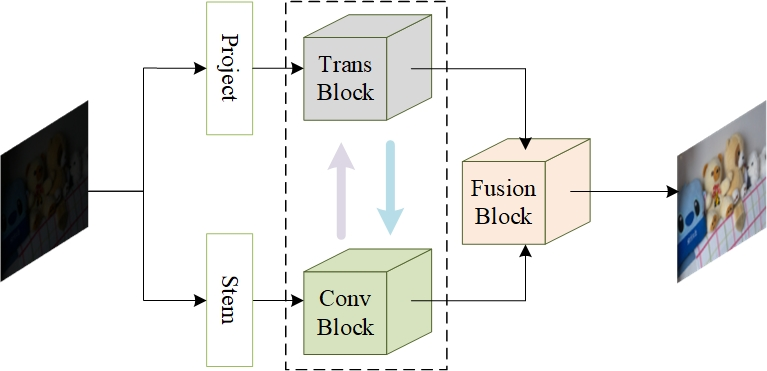
\includegraphics[width=\linewidth]{picture/LLIE/My Architecture/The proposed initial architecture(Abstract Picture)}
			\captionsetup{font=scriptsize}
			\caption{Thumbnail of PACUT}
			\label{fig: The proposed initial architecture(Abstract Picture)}	
		\end{subfigure}
		%\captionsetup{font=scriptsize}
		\caption{
			\label{fig: PACUT}
			我们提出的初步恢复图架构。图\ref{fig: First Architecture} CNN 分支和 Transformer 分支以及 FCU (Feature Coupling Unit)。图\ref{fig: Up-sampling and down-sampling} 特征映射和 Patch embeddings 空间对齐的上采样和下采样过程。 图\ref{fig: The proposed initial architecture(Abstract Picture)} PACUT 的缩略图。PACUT 结构受 Conformer\cite{peng2021conformer}启发,将原来结构中 CNN 分支的 ResNet 结构修改为 U-Net 结构。其采用一个 U-Net 和 ViT 的并行架构,通过 U-Net 结构得到一个弱恢复的弱特征图 $\mathcal{F}_2$,通过 ViT 融合的特征可以初步增强弱特征图 $\mathcal{F}_2$,ViT 的输出经过 Patch Expanding 的特征图 $\mathcal{F}_3$ 经过与 U-Net 输出的特征图 $\mathcal{F}_2$ 融合之后得到一个初步恢复的图片 output image,用以后续参与图片的进一步恢复。
		}
	\end{figure}
	\FloatBarrier
	
	在计算机视觉领域,图像特征的研究通常聚焦于两个主要方面:局部特征\cite{jain1991unsupervised, lowe2004distinctive, ojala2002multiresolution}和全局特征\cite{lisin2005combining}。局部特征是对图像微小区域的紧凑向量描述,而全局特征则涵盖更广泛的范围,包括长距离轮廓、形状描述符和不同对象类别的识别
	
	在深度学习框架下,卷积神经网络(CNN)通过卷积操作逐步提取图像的局部特征,而视觉变换器(Vision Transformers)采用自注意力模块以更灵活的方式聚合这些特征,形成对整体图像的全面理解。这在处理全局特征时显示出显著优势,特别是在捕获长距离依赖关系和整体图像结构方面。
	
	在初步恢复图的图像增强方面,我们受到了结合了卷积神经网络和Transformer自注意力模块的Conformer\cite{peng2021conformer}结构的启发。为了克服Transformer在捕获远距离特征时可能忽视局部特征细节的局限性,我们提出了一种并行深度学习架构,旨在提升弱光图像增强任务中恢复图像的可视性和质量,同时保留关键的细节和纹理\cite{karu1996there}信息,如图\ref{fig: PACUT}所示。
	
	该架构包括两个并行分支、一个Stem模块、一个特征连接单元(FCU)和一个融合模块。Stem模块\cite{szegedy2016rethinking}提取图像的初始局部特征,将其输入到CNN分支。CNN分支采用改进的U-Net结构,而Transformer分支由修改后的 Vision Transformer 组成。FCU作为桥接模块,融合两个分支的局部特征和全局表征。最终,两个分支的输出通过特征融合模块生成最终的增强图像。在训练中,我们采用结合$\mathcal{L}_1$和SSIM损失函数的策略进行优化。
	
	\subsubsection{边缘检测网络}
	
	边缘检测是视觉任务中非常基础的任务,现有的基于 CNN 的边缘检测方法有两个明显的问题。
	
	\begin{itemize}
		\item [(1)] 首先,当前大多数方法主要依赖于 CNN 的最终层(通常是最后一层卷积层)的输出,而忽视了网络中间层的潜在价值。这种做法可能导致信息的丢失,特别是那些在中间层中更为显著的特征信息。
		
		\item [(2)] 虽然研究者们普遍关注于探索更深层次的 CNN 结构,但在边缘检测这一特定任务中,这种方法面临着数据稀缺性和梯度消失问题的双重挑战。由于边缘检测任务通常涉及的数据量相对较少,加之深层网络易于出现梯度消失,这些因素共同制约了深层 CNN 在边缘检测领域的应用效果。
	\end{itemize}
	
	\begin{figure}[htb]
		\centering
		\begin{subfigure}{0.19\textwidth}
			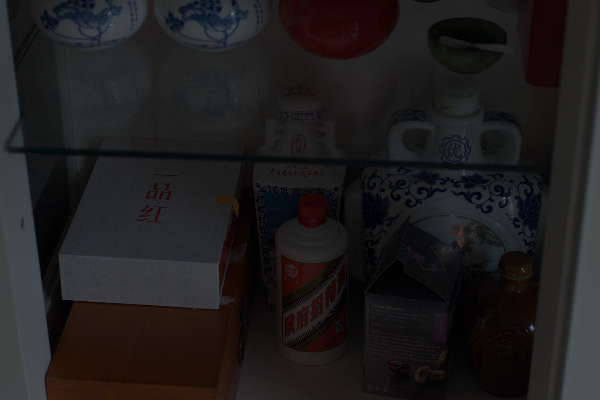
\includegraphics[width=\linewidth]{picture/LLIE/My Architecture/Edge Detection/low00044}
			\captionsetup{font=scriptsize}
			\caption{LLI}
			\label{fig: LLI}
		\end{subfigure}
		\begin{subfigure}{0.19\textwidth}
			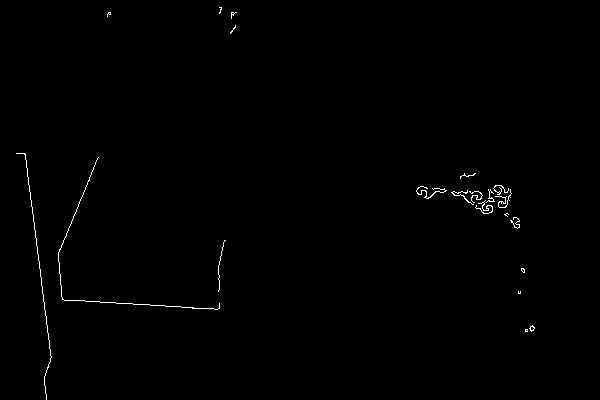
\includegraphics[width=\linewidth]{picture/LLIE/My Architecture/Edge Detection/low00044_canny}				
			\captionsetup{font=scriptsize}
			\caption{LLI Canny}
			\label{fig: LLI_canny}	
		\end{subfigure}
		\begin{subfigure}{0.19\textwidth}
			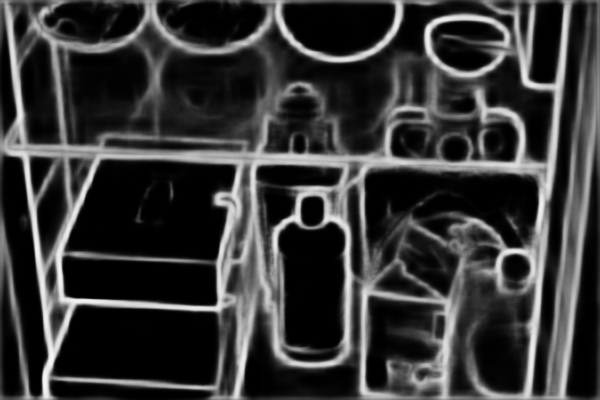
\includegraphics[width=\linewidth]{picture/LLIE/My Architecture/Edge Detection/low00044_rcf}
			\captionsetup{font=scriptsize}
			\caption{LLI RCF}
			\label{fig: LLI_rcf}
		\end{subfigure}
		\begin{subfigure}{0.19\textwidth}
			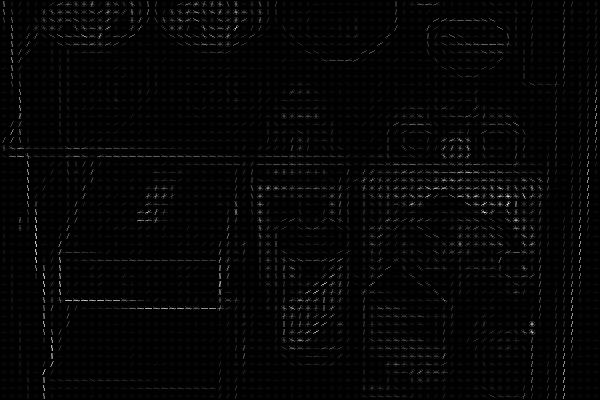
\includegraphics[width=\linewidth]{picture/LLIE/My Architecture/Edge Detection/low00044_hog}
			\captionsetup{font=scriptsize}
			\caption{LLI HOG}
			\label{fig: LLI_hog}
		\end{subfigure}
		\begin{subfigure}{0.19\textwidth}
			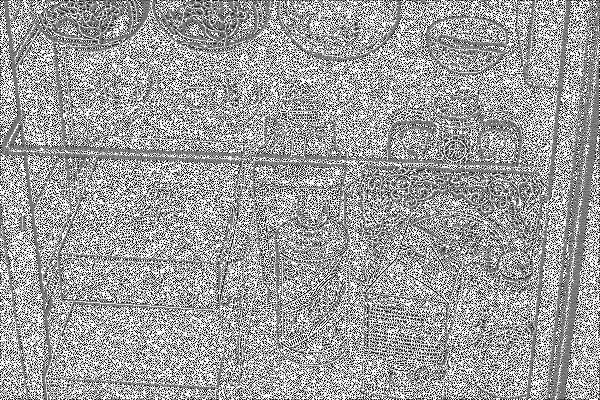
\includegraphics[width=\linewidth]{picture/LLIE/My Architecture/Edge Detection/low00044_lbp}
			\captionsetup{font=scriptsize}
			\caption{LLI LBP}
			\label{fig: LLI_lbp}
		\end{subfigure}\\
		\begin{subfigure}{0.19\textwidth}
			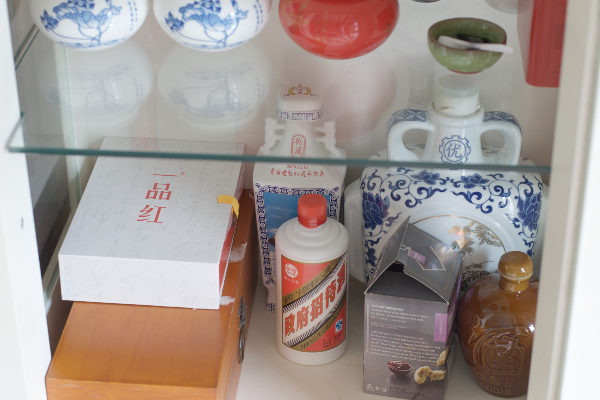
\includegraphics[width=\linewidth]{picture/LLIE/My Architecture/Edge Detection/normal00044}
			\captionsetup{font=scriptsize}
			\caption{GT}
			\label{fig: GI}
		\end{subfigure}
		\begin{subfigure}{0.19\textwidth}
			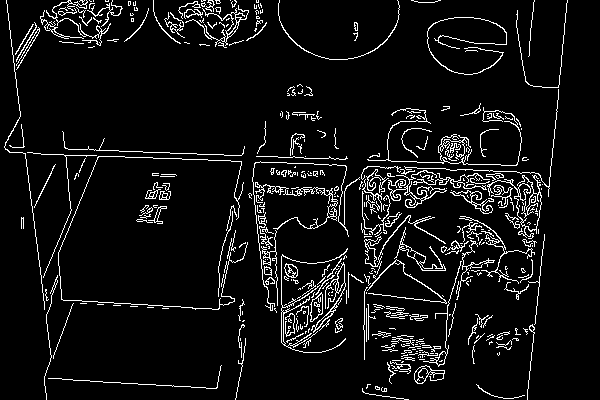
\includegraphics[width=\linewidth]{picture/LLIE/My Architecture/Edge Detection/normal00044_canny}
			\captionsetup{font=scriptsize}
			\caption{GT Canny}
			\label{fig: GT_canny}
		\end{subfigure}
		\begin{subfigure}{0.19\textwidth}
			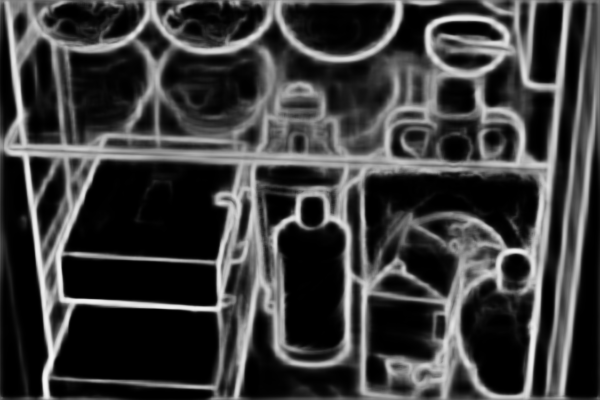
\includegraphics[width=\linewidth]{picture/LLIE/My Architecture/Edge Detection/normal00044_rcf}
			\captionsetup{font=scriptsize}
			\caption{GT RCF}
			\label{fig: GT_rcf}
		\end{subfigure}
		\begin{subfigure}{0.19\textwidth}
			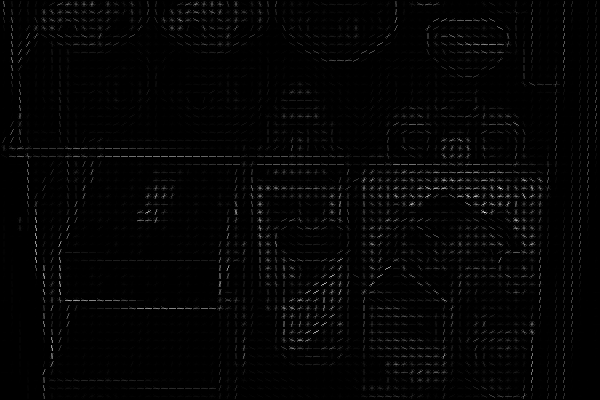
\includegraphics[width=\linewidth]{picture/LLIE/My Architecture/Edge Detection/normal00044_hog}
			\captionsetup{font=scriptsize}
			\caption{GT HOG}
			\label{fig: GT_hog}	
		\end{subfigure}
		\begin{subfigure}{0.19\textwidth}
			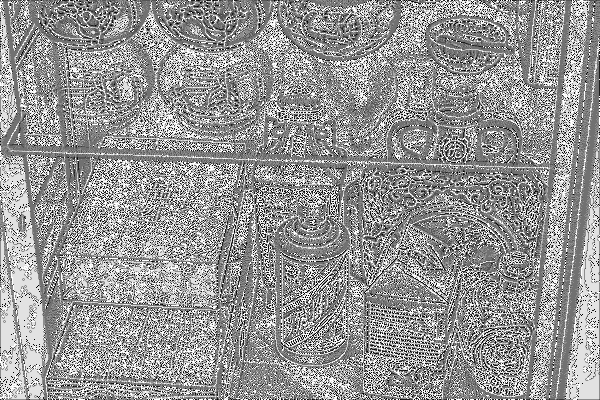
\includegraphics[width=\linewidth]{picture/LLIE/My Architecture/Edge Detection/normal00044_lbp}
			\captionsetup{font=scriptsize}
			\caption{GT LBP}
			\label{fig: GT_lbp}	
		\end{subfigure}
		\caption{
			\label{fig: LLI Structure Information}
			基于 LOL-v2 弱光数据集的边缘信息。
		}
	\end{figure}
	
	Liu\cite{liu2017richer}发现不同卷积层获得的结果随着深度增加而更加粗糙,其提出 RCF(Richer convolutional features) 方法充分利用所有 CNN 层的结果。相比之下,HED (Holistically-nested edge detection) \cite{xie2015holistically}方法仅采用了 VGG16 架构中每个阶段的最后一层卷积输出,而 RCF (Richer Convolutional Features) 方法则利用了每个层级的卷积结果。这一策略使得 RCF 在捕获丰富的边缘信息方面展现了更为显著的能力。
	
	此外,获取边缘图的方法也各不相同,在 LLIE 任务中,常见方法采用边缘检测网络来生成边缘图,然后使用 Canny 或 Sobel 算子\cite{maini2009study}从 GT 中获取边缘图用做对照组。目前在 LLIE 领域中获取边缘图分化成了两个不同的方向,一种是通过初步恢复图像获取边缘图(见图\ref{fig: EEMEFN}),另一种是直接通过弱光图像以获取边缘图(见图\ref{fig: EdgeNet})。LLIE 任务中边缘检测的主要有下列方法:
	
	在LLIE(低光照图像增强)任务中,边缘检测技术的应用可概括为以下几种主要方法:
	
	\begin{itemize}
		\item [(1)] 利用手工设计的各类滤波器生成边缘图像。
		
		\item [(2)] 采用基于人类设计特征的数据驱动模型(如使用随机决策森林)来预测边缘。
		
		\item [(3)] 通过深度学习技术,从原始数据中学习复杂的特征表示,实现端到端的边缘检测模型(例如RCF边缘检测模型\cite{liu2017richer})。
	\end{itemize}
	
	经过广泛的文献综述,我们发现在LLIE领域内,边缘图像的获取主要分为两个不同的路径:一是从初步恢复的图像中提取边缘图(如图\ref{fig: EEMEFN}所示),二是直接从低光照图像中提取边缘图(如图\ref{fig: EdgeNet}所示)。传统方法如 Canny 和 Sobel 算子\cite{maini2009study}在直接从低光照图像中提取边缘时面临较大挑战,如图\ref{fig: LLI_canny}所示。然而,基于深度学习的方法能从低光照图像中提取出更为详细的边缘图像,虽然与真实边缘仍有差异。我们的研究目标是缩减这一差距,以提高基于结构建模指导的模型的准确性。本研究尝试使用不同曝光度的图片,获取它们的 HOG 和 LBP 图像,并采用多曝光图像融合架构,从而获得更接近真实边缘结构的边缘图像,其结构示意见图\ref{fig: Edge Detection Network}。
	
	%现在的方法大多只使用 CNN 的最后一层 conv 的结果,忽略了中间层的结果。
	
	%更多的方法集中在探究更深的 CNN,但边缘检测是数据比较少,而且容易发生梯度消失的现象。
	
	\begin{figure}[htb]
		% read manual to see what [ht] means and for other possible options
		\centering 
		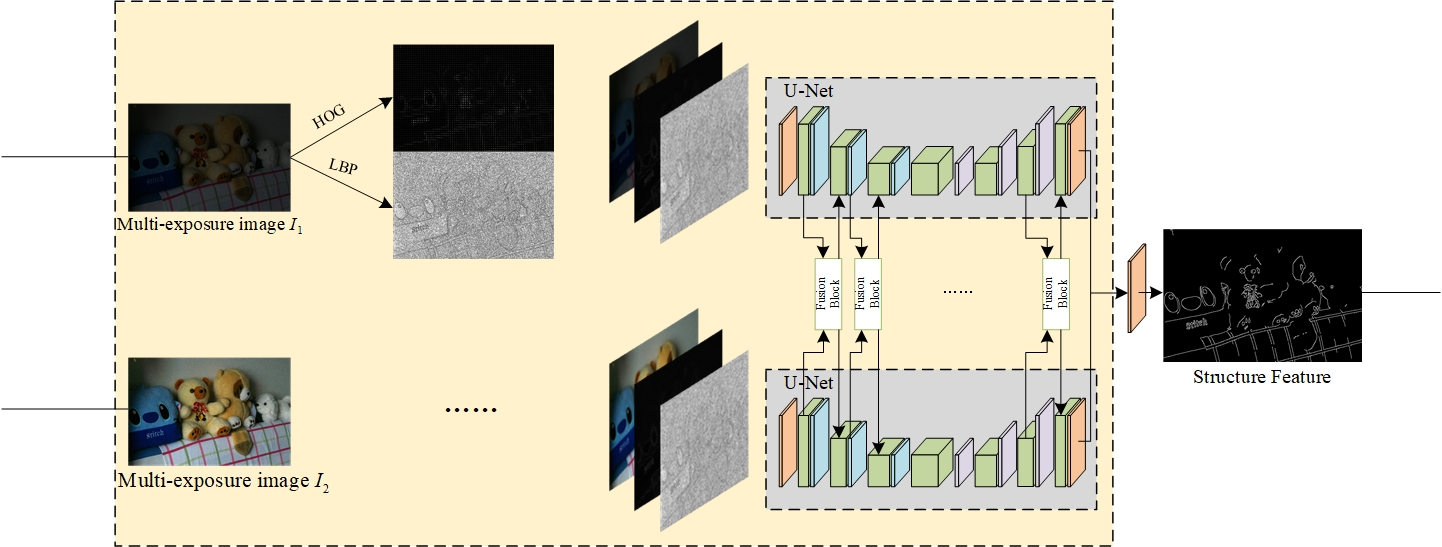
\includegraphics[width=\columnwidth]{picture/LLIE/My Architecture/Edge Detection Network}
		%\captionsetup{font=scriptsize}
		\caption{
			\label{fig: Edge Detection Network} 
			边缘检测网络。
		}
	\end{figure}
	\FloatBarrier
	
	\subsection{计划进度}

	\begin{table}[!htbp]
		\centering
		%\resizebox{\textwidth}{!}{ %按照宽度调整调整表格大小
			\begin{tabular}{ccc}
				\toprule
				阶段  & 任务描述                                                & 计划完成时间 \\
				\midrule
				阶段1 & 继续收集文献,深入了解研究领域        	                 & 1月-2月     \\
				阶段2 & 继续明确研究问题和目标,并确定具体的方法                   & 3月-4月     \\
				阶段3 & 进行相关文献的代码复现,用于后续的对比实验                 & 5月-6月     \\
				阶段4 & 构建模型,进行实验                                       & 7月-8月     \\
				阶段5 & 数据分析,初步整理实验结果                                & 9月-10月    \\
				阶段6 & 撰写论文,准备答辩相关材料                                & 11月-12月   \\
				\bottomrule
			\end{tabular}
		%}
		%\captionsetup{font=scriptsize} %设置标题字体与表格字体一致
		\caption{
			\label{tab: Schedule}
			计划进度
		} 
	\end{table}
	
	\subsection{预期的研究进展}
	
	接下来主要工作主要从以下方面开展:
	
	通过完善文献调研工作进一步阐述弱光图像恢复的重要性及其在当前研究领域的挑战性,包括强调边缘信息在图像处理中的关键作用。此外,进一步明确提出研究的主要目标。综述现有文献,包括边缘检测技术、低光图像恢复方法以及Transformer网络的应用。分析现有方法的局限性,并探讨潜在的改进方向。
	
	总结下来分为以下三个方面:
	\begin{itemize}
		\item[(1)] \textbf{边缘检测网络评价指标的研究:}确立用于评估边缘检测网络性能的关键指标,如精度、召回率和F1分数等。此外,设计实验以量化评估不同边缘检测方法在低光条件下的表现。
		
		\item[(2)] \textbf{实验设计与验证:}使用现有边缘检测模型(例如RCF)进行初步实验,评估其在弱光图像恢复中的效果。对比分析现有技术与改进方法的性能差异。
		
		\item[(3)] \textbf{改进方案的探索与实现:}尝试结合 RCF 方法和 Transformer 模型,设计新的边缘检测与图像恢复模型,并在标准数据集上测试新模型,并与传统方法进行性能比较。
	\end{itemize}
	
	\section{课题的创新性}
	
	我们拟在现有研究基础上对弱光图像增强模型进行关键改进,以提升其性能。具体创新点包括:
	
	\begin{itemize}
		\item [(1)] 深度卷积网络(CNN) 分支:该分支基于 U-Net 架构,采用多层卷积神经网络,通过逐层提取图像的局部特征来增强图像的细节和纹理。此分支的设计旨在处理图像的低级特征,如边缘、纹理和颜色信息。
		
		\item [(2)] Vision Transformer (ViT) 分支:该分支利用了Vision Transformer 的能力,通过自注意力机制捕捉图像的长距离依赖关系。ViT 分支专注于提取图像的全局特征,如整体结构和上下文信息。
		
		\item [(3)] 特征耦合单元 (FCU):为了有效地融合CNN 分支和ViT 分支的特征,引入了特征耦合单元(FCU)。FCU 通过下采样(FCUDown) 和上采样(FCUUp) 操作,实现了CNN 特征图和Transformer patch embeddings 之间的无缝转换,从而实现了局部特征和全局表示的连续耦合。
		
		\item [(4)] 构建一种有效的从弱光图像中生成边缘图的边缘网络
		
		\item [(5)] 构建一种能够的解决弱光图像中的局部边缘失真问题的模型
	\end{itemize}
	
	这些关键改进旨在深化对弱光图像增强的理解,并为解决现有模型的局限性提供新的途径。
	
	\section{研究基础}
	
	\subsection{已完成工作}
	
	\subsubsection{初步恢复图像的生成模型实验结果}
	
	我们通过实验验证了初步恢复图像的生成模型,验证了提出方法的有效性。首先介绍了实验细节,包括网络实现、数据集和评估指标。通过与领先技术比较,展示了我们网络在低光图像增强任务中的性能。消融研究探讨了各组件在任务中的作用和重要性的相对重要性和功能。通过系统地移除或修改网络的特定部分,我们能够评估每个组件对最终增强效果的贡献,从而深入理解整个网络的工作机制。这些实验结果为我们的网络设计提供了进一步的洞察和验证。
	
	\subsubsection{数据集和评价指标}
	
	我们对LOL\cite{wei2018deep}和SCIE\cite{cai2018learning}两个公共数据集进行了实验评估,以全面评估提出网络的性能。评估过程中使用了峰值信噪比(PSNR)\cite{wang2004image}、结构相似度(SSIM)\cite{wang2004image}和自然图像质量评估器(NIQE)\cite{mittal2012making}等度量指标,客观评估图像增强结果的质量,深入了解提出网络在低光照环境下的性能表现。
	
	\subsubsection{对比试验}
	
	我们将所提算法的结果与多个公开可获得的代码进行比较,包括HE\cite{pisano1998contrast}、LightenNet\cite{li2018lightennet}、LLNet\cite{lore2017llnet}、Retinex-Net\cite{wei2018deep}、MBLLEN\cite{lv2018mbllen}、EnlightenGAN\cite{jiang2021enlightengan}、Zero-DCE\cite{guo2020zero}以及KinD\cite{zhang2019kindling}。
	
	\begin{table}[!htbp]
		\centering
		\tiny
		\resizebox{\textwidth}{!}{ %按照宽度调整调整表格大小
				\begin{tabular}{>{\centering\arraybackslash}m{2.5cm}|c|c|c|c|c|c}
						
						\hline %添加表格头部粗线
						
						\multirowcell{2}{\textbf{Method}} & \multicolumn{3}{c|}{\makecell{\textbf{LOL}\cite{wei2018deep}}} & \multicolumn{3}{c}{\makecell{\textbf{SCIE}\cite{cai2018learning}}} \\
						
						\cline{2-7}
						
						
						      & \textbf{PSNR↑} & \textbf{SSIM↑} & \textbf{NIQE↓} & \textbf{PSNR↑}  & \textbf{SSIM↑} & \textbf{NIQE↓} \\
						
						\hline
						
						input & 7.773 & 0.181 & 0.560 & 17.824 & 0.779 & 0.148  \\
						
						\hline	
						
						HE\cite{pisano1998contrast}             & 15.467 & 0.504 & 9.531 & 15.342 & 0.741 & 9.232 \\
						LightenNet\cite{li2018lightennet}       & 10.301 & 0.361 & 7.422 & 13.579 & 0.744 & 8.166 \\
						LLNet\cite{lore2017llnet}               & \textcolor{blue}{17.953} & 0.704 & \textcolor{red}{3.974} & 12.177 & 0.645 & 4.292 \\
						Retinex-Net\cite{wei2018deep}           & 16.774 & 0.462 & 5.474 & 12.310 & 0.671 & 7.239 \\ 
						KinD\cite{zhang2019kindling} 	          & 16.648 & \textcolor{blue}{0.779} & 6.175 & 21.103 & \textcolor{red}{0.838} & 4.195 \\
						MBLLEN\cite{lv2018mbllen}               & 17.902 & 0.715 & \textcolor{blue}{4.247} & 13.638 & 0.632 & \textcolor{blue}{2.108} \\
						EnlightenGAN\cite{jiang2021enlightengan}& 17.483 & 0.658 & 4.889 & 18.726 & 0.822 & 5.216 \\
						Zero-DCE\cite{guo2020zero}              & 17.622 & 0.556 & 7.972 & \textcolor{red}{22.682} & 0.810 & \textcolor{red}{1.158} \\
						\textbf{Ours}                             & \textcolor{red}{22.780} & \textcolor{red}{0.823} & 4.473 & \textcolor{blue}{21.543} & \textcolor{blue}{0.835} & 3.412 \\
						\hline
						
					\end{tabular}
			}
		%\captionsetup{font=scriptsize} %设置标题字体与表格字体一致
		\caption{
				\label{tab: Quantitative Comparisons on LOL-test and SCI testing datasets}
				LOL和SCIE数据集在各方法下的对比值,其中红色表示最优,蓝色表示次优,$↑$表示越高越好,$↓$表示越低越好。
				} 
	\end{table}
	
	本研究通过对 LOL 数据集的全面评估展示了所提出模型与其他方法的整体性能,具体结果见表\ref{tab: Quantitative Comparisons on LOL-test and SCI testing datasets}。在LOL测试数据集上,我们的模型展现出卓越的性能,其 PSNR 和 SSIM 达到最佳水平。在 SCIE 测试数据集上,尽管 PSNR 和 SSIM 相对较低,但仍表现出令人满意的效果,验证了模型的有效性。
	
	\begin{figure}[htb] 
		\centering 
		\begin{subfigure}{0.19\textwidth}
			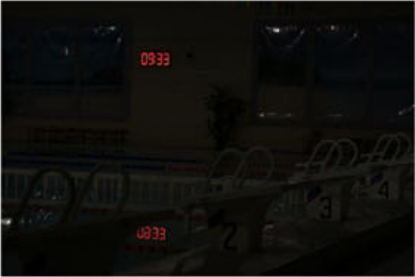
\includegraphics[width=\linewidth]{picture/LLIE/Efficent/Input}
			\captionsetup{font=scriptsize}
			\caption{Input}
			\label{fig: LLI Input}
		\end{subfigure}
		\begin{subfigure}{0.19\textwidth}
			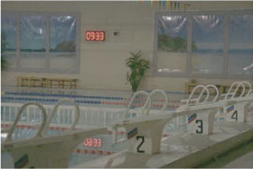
\includegraphics[width=\linewidth]{picture/LLIE/Efficent/LightenNet}
			\captionsetup{font=scriptsize}
			\caption{LightenNet}
			\label{fig: LightenNet}
		\end{subfigure}
		\begin{subfigure}{0.19\textwidth}
			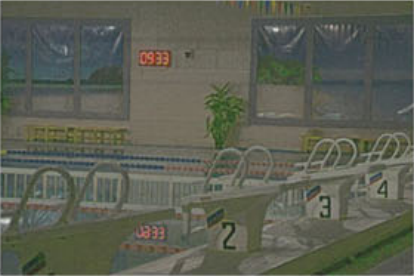
\includegraphics[width=\linewidth]{picture/LLIE/Efficent/LLNet}				
			\captionsetup{font=scriptsize}
			\caption{LLNet}
			\label{fig: LLI LLNet}	
		\end{subfigure}
		\begin{subfigure}{0.19\textwidth}
			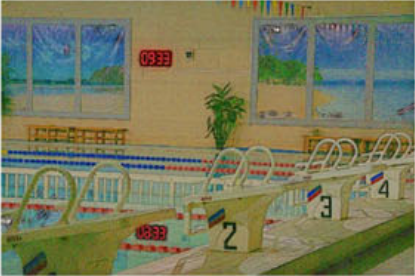
\includegraphics[width=\linewidth]{picture/LLIE/Efficent/RetinexNet}
			\captionsetup{font=scriptsize}
			\caption{RetinexNet}
			\label{fig: LLI RetinexNet}	
		\end{subfigure}
		\begin{subfigure}{0.19\textwidth}
			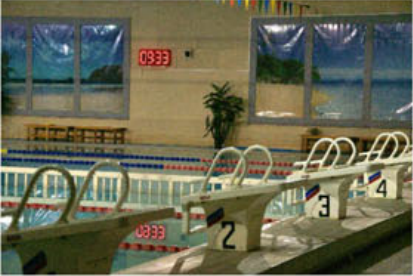
\includegraphics[width=\linewidth]{picture/LLIE/Efficent/KinD}
			\captionsetup{font=scriptsize}
			\caption{KinD}
			\label{fig: KinD}	
		\end{subfigure}\\
		\begin{subfigure}{0.19\textwidth}
			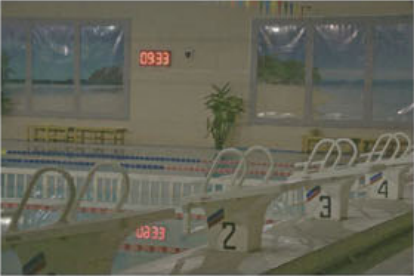
\includegraphics[width=\linewidth]{picture/LLIE/Efficent/MBLLEN}
			\captionsetup{font=scriptsize}
			\caption{MBLLEN}
			\label{fig: MBLLEN}	
		\end{subfigure}
		\begin{subfigure}{0.19\textwidth}
			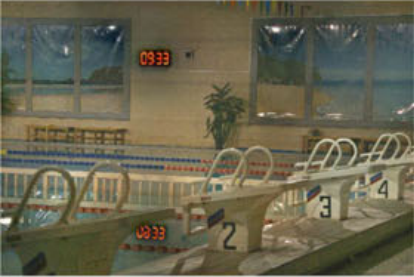
\includegraphics[width=\linewidth]{picture/LLIE/Efficent/EnlightenGAN}
			\captionsetup{font=scriptsize}
			\caption{EnlightenGAN}
			\label{fig: LLI EnlightenGAN}	
		\end{subfigure}
		\begin{subfigure}{0.19\textwidth}
			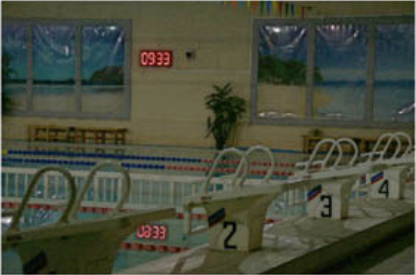
\includegraphics[width=\linewidth]{picture/LLIE/Efficent/Zero-DCE}
			\captionsetup{font=scriptsize}
			\caption{Zero-DCE}
			\label{fig: Zero-DCE}	
		\end{subfigure}
		\begin{subfigure}{0.19\textwidth}
			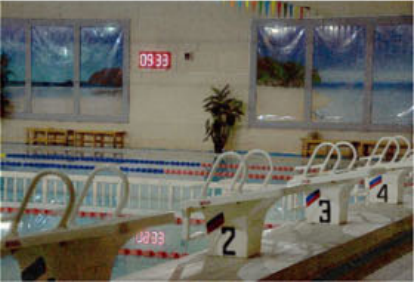
\includegraphics[width=\linewidth]{picture/LLIE/Efficent/Ours}
			\captionsetup{font=scriptsize}
			\caption{Ours}
			\label{fig: Ours}	
		\end{subfigure}
		\begin{subfigure}{0.19\textwidth}
			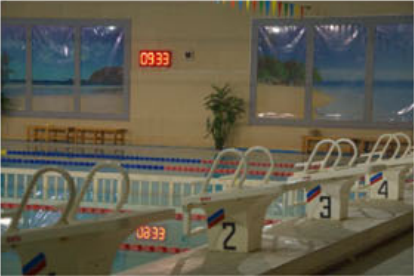
\includegraphics[width=\linewidth]{picture/LLIE/Efficent/GT}
			\captionsetup{font=scriptsize}
			\caption{GT}
			\label{fig: GT}	
		\end{subfigure}
		%\captionsetup{font=scriptsize}
		\caption{
			\label{fig: LOL}
			不同方法在LOL测试数据集上的视觉表现。
		}
	\end{figure}
	
	图\ref{fig: LOL}展示了各种方法在LOL测试数据集上的图像增强效果,其中 GT 表示真实图片。与Zero-DCE、LLNet和MBLLEN相比,RetinexNet呈现出颜色饱和度更强的增强效果,而Zero-DCE、LLNet和MBLLEN的结果在视觉上偏暗。EnlightenGAN在增强的图像中显示出明显的灰色伪影,表明其对噪声较为敏感。尽管我们的方法相对真实值而言稍显偏亮,但在LOL数据集上表现出优于对比方法的效果。
	
	\subsubsection{消融实验}
	
	我们采用PSNR、SSIM和NIQE指标,对SCConv模块、Transformer分支以及基于不同尺寸的预训练视觉变换器模型的有效性进行评估。我们设定去除SCConv模块的CNN分支作为基线网络。如表\ref{tab: Ablation Study}所示,引入Transformer分支并增加输入到Transformer分支的特征图尺寸,相较于基线,模型性能得到了显著改善。
	
	\begin{table}[!htbp]
		\centering
		\tiny
		\resizebox{\textwidth}{!}{ %按照宽度调整调整表格大小
			\begin{tabular}{c|c|c|c|c|c|c}
						
					\hline
						
					\textbf{基线模型} & \textbf{SCConv} & \textbf{Transformer分支} & \textbf{Transformer预训练权重尺寸}  & \textbf{PSNR↑} & \textbf{SSIM↑} & \textbf{NIQE↓} \\
			
					\hline
					
					\checkmark &            &            &                  & 18.222 & 0.642 & 7.213 \\
					\checkmark & \checkmark &            &                  & 18.231 & 0.523 & 5.231 \\
					\checkmark & \checkmark & \checkmark & $224 \times 224$ & 21.643 & 0.815 & 4.552 \\
					\checkmark & \checkmark & \checkmark & $384 \times 384$ & \textbf{22.780} & \textbf{0.823} & \textbf{4.473} \\
		
					\hline			
			\end{tabular}
		}
		%\captionsetup{font=scriptsize} %设置标题字体与表格字体一致
		\caption{
			\label{tab: Ablation Study}
			Transformer分支和Transformer预训练权重尺寸和SCConv对模型的影响。
		} 
	\end{table}

\end{document}
